\section{Hypothesentest}\label{nullhypothese}
\begin{enumerate}[nosep]
	\item Nullhypothese $H_0$ formulieren
	\item Messgrössen bestimmen, mit der $H_0$ getestet werden kann (Teststatistik)
	\item Verteilung der Messgrössen ermitteln
	\item Paramter der Verteilung schätzen
	\item Kritischen Wert für die Testgrösse bestimmen, der nur mit Wahrscheinliche $\alpha$ überschritten wird
	\item Ist die Messgrösse im vorliegenden Experiment unwahrscheinliche hoch? $\xRightarrow[]{} H_0$ verwerfen
\end{enumerate}

Die Nullhypothese $H_0$ und die Alternativhypothese $H_1$ sind gegensätzlich, wobei die Grunsatzfrage beantworten werden muss. \\
\textbf{Schlechtes Beispiel:} $H_0$: Das Medikament hat keine Wirkung. \textit{vs} $H_1$: Das Medikament hat eine Wirkung. (Beantwortet die Frage nicht)

\subsection{Fehlerarten}
\textbf{Art 1:} Nullhypothese verworfen, obwohl wahr (zufallsbedingt unwahrscheindlicher Wert der Teststatistik, falsch positives Ergebnis). \textbf{Art 2:} Nullhypotese nicht verworfen, obwohl falsch (falsches Negatives Ergebnis). Übliche Werte für Fehler Art 1:
\begin{center} 
	\begin{tabular}{ll}
	$\alpha$ & \\ \hline
	0.05 & Signifikant \\ \hline
	0.01 & \multirow{2}{*}{Hoch Signifikant} \\
	0.01 &  \\ \hline
\end{tabular}
\end{center}

\subsection{t-Test}
Die Stichproben $X_1...X_n$ und $Y_1...Y_n$ mit gleicher Varianz haben den gleichen Erwartungswert. Die Teststatistik ergibt sich aus der t-verteilt mit $m+n-2$ Freiheitsgraden.
\[
t = \frac{\overline{X} - \overline{Y}}{\sqrt{(n -1)S^2_X + (m -1)S^2_Y}}\sqrt{\frac{mn(n+m-2)}{n+3}}
\]

Varianz muss geschätzt werden, analog auch für $Y$:
\[
\overline{X} = \frac{X_1 + \dots + X_n}{n}, \qquad S^2_X = \frac{1}{n-1}\sum_{i=1}^{n}(X_i - \overline{X})^2
\]


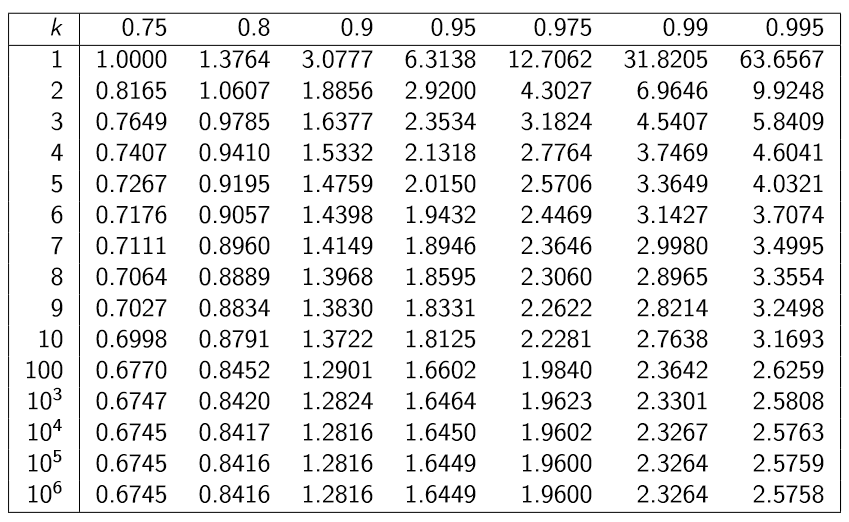
\includegraphics[width=\columnwidth]{Images/t-tabelle}


\section{Testen einer Verteilung}
\subsection{$\chi^2$ Test}
\todo{Woche 12}
Um eine diskrete Verteilung $P(X = x_i) = p_i$ mit $n_i$ Beobachtungen zu testen wird die Nullhypothese $H_0$ (Siehe Kapitel \ref{nullhypothese}) überprüft. Die Diskrepanz $D$ wird dabei wie folgt berechnet:
\[
D = \sum_{i=1}^{k}\frac{(n_i - np_i)^2}{np_i}
\]
Anschliessend wird die $\chi^2$-Verteilung mit $k-1$ Freiheitsgraden berechnet. Die benötigten Parameter können via Schätzung (Siehe Kapitel \ref{schaetzen}) oder Messung bestimmt werden. Damit lässt sich der kritische Wert $D_\text{krit}$ aus der $\chi^2$-Tabelle bestimmen. $H_0$ wird verworfen, wenn $D > D_\text{krit}$ ist.

\subsubsection{$\chi^2$ Tabelle}
Achtung: $\alpha = 1 - p_i$\\
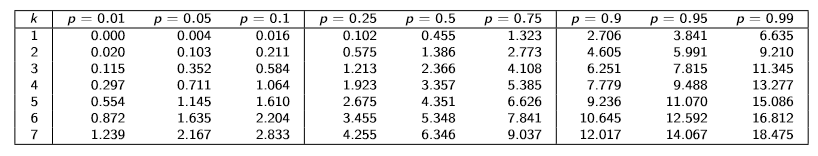
\includegraphics[width=\columnwidth]{Images/chi-tabelle}

\subsubsection{$\chi^2$ Verteilung}\label{chi-verteilung}
Wenn Diskrepanz\\
$D>D_+ \Rightarrow$ Daten passen nicht ($H_0$ verwerfen)\\
$D < D_- \Rightarrow$ Daten passen zu gut (Hinweis auf Betrug)
\begin{center}
	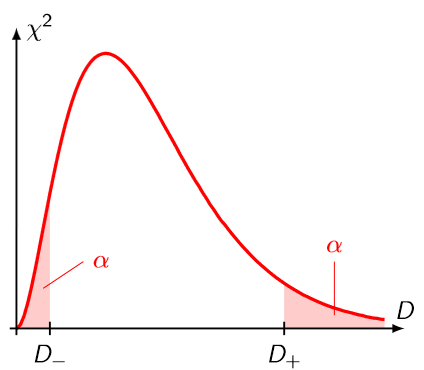
\includegraphics[width=0.6\columnwidth]{Images/chi-verteilung}
\end{center}

\noindent\textbf{Beispiel}: Siehe Kapitel \ref{tictac}
\\
\noindent\textbf{ACHTUNG}: Wenn nur wenige Messungen am Anfang bzw Ende $<5$ der Verteilung vorliegen, sollte der Kolmogorov-Smirnov-Test verwendet werden.
\begin{center}
	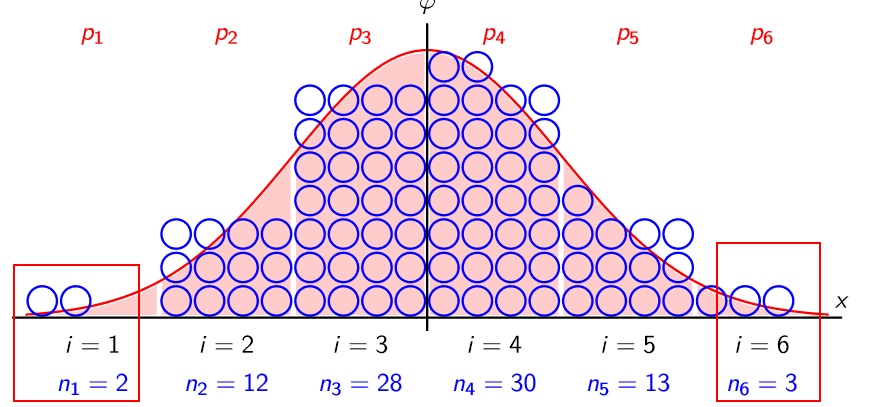
\includegraphics[width=0.4\columnwidth]{Images/chi-verteilung-fail}
\end{center}

\subsection{Kolmogorov-Smirnov-Test}
Um eine stetige Verteilung zu testen kann der Kolmogorov-Smirnov-Test verwendet werden. Dazu werden die Ergebnisse von klein nach gross sortiert. $F(x)$ ist die Verteilung, welche überprüft werden soll. 

\begin{align*}
	K_n^+ &= \sqrt{n}\max\left(\frac{j}{n} - F(x_j)\right) \\
	K_n^- &= \sqrt{n}\max\left(F(x_j) - \frac{j-1}{n}\right) \\
\end{align*}

\textbf{Beispiel:} Siehe Kapitel \ref{Kolmogorov}

\subsubsection{K-Tabelle}
Achtung: $\alpha = 1 - p_i$\\
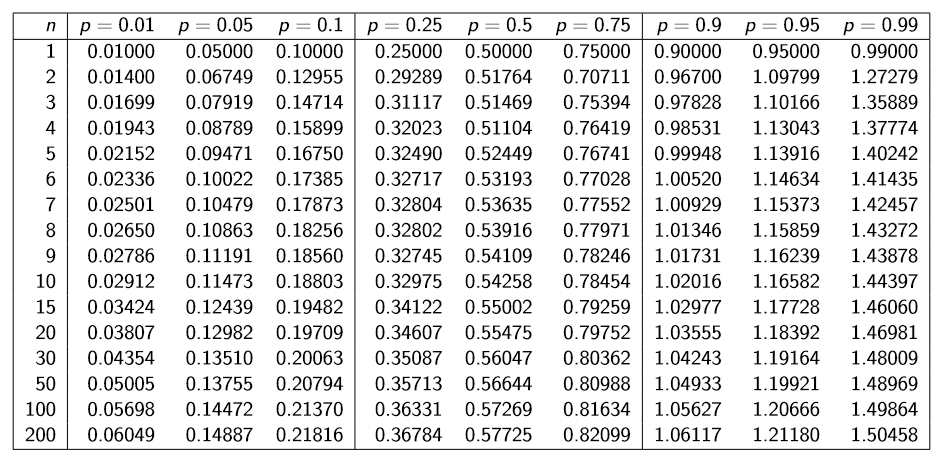
\includegraphics[width=\columnwidth]{Images/ktabelle}
